\chapter{济南市丁家庄城中村照片集}
\thispagestyle{empty}
本章图片均为笔者拍摄于丁家庄城中村,采用了如实摄影(straight photography)的拍摄
手法,力图直接呈现丁家庄的生态,让其为自己发声。

\vspace{2cm}
\begin{figure}[!ht]
  \centering
  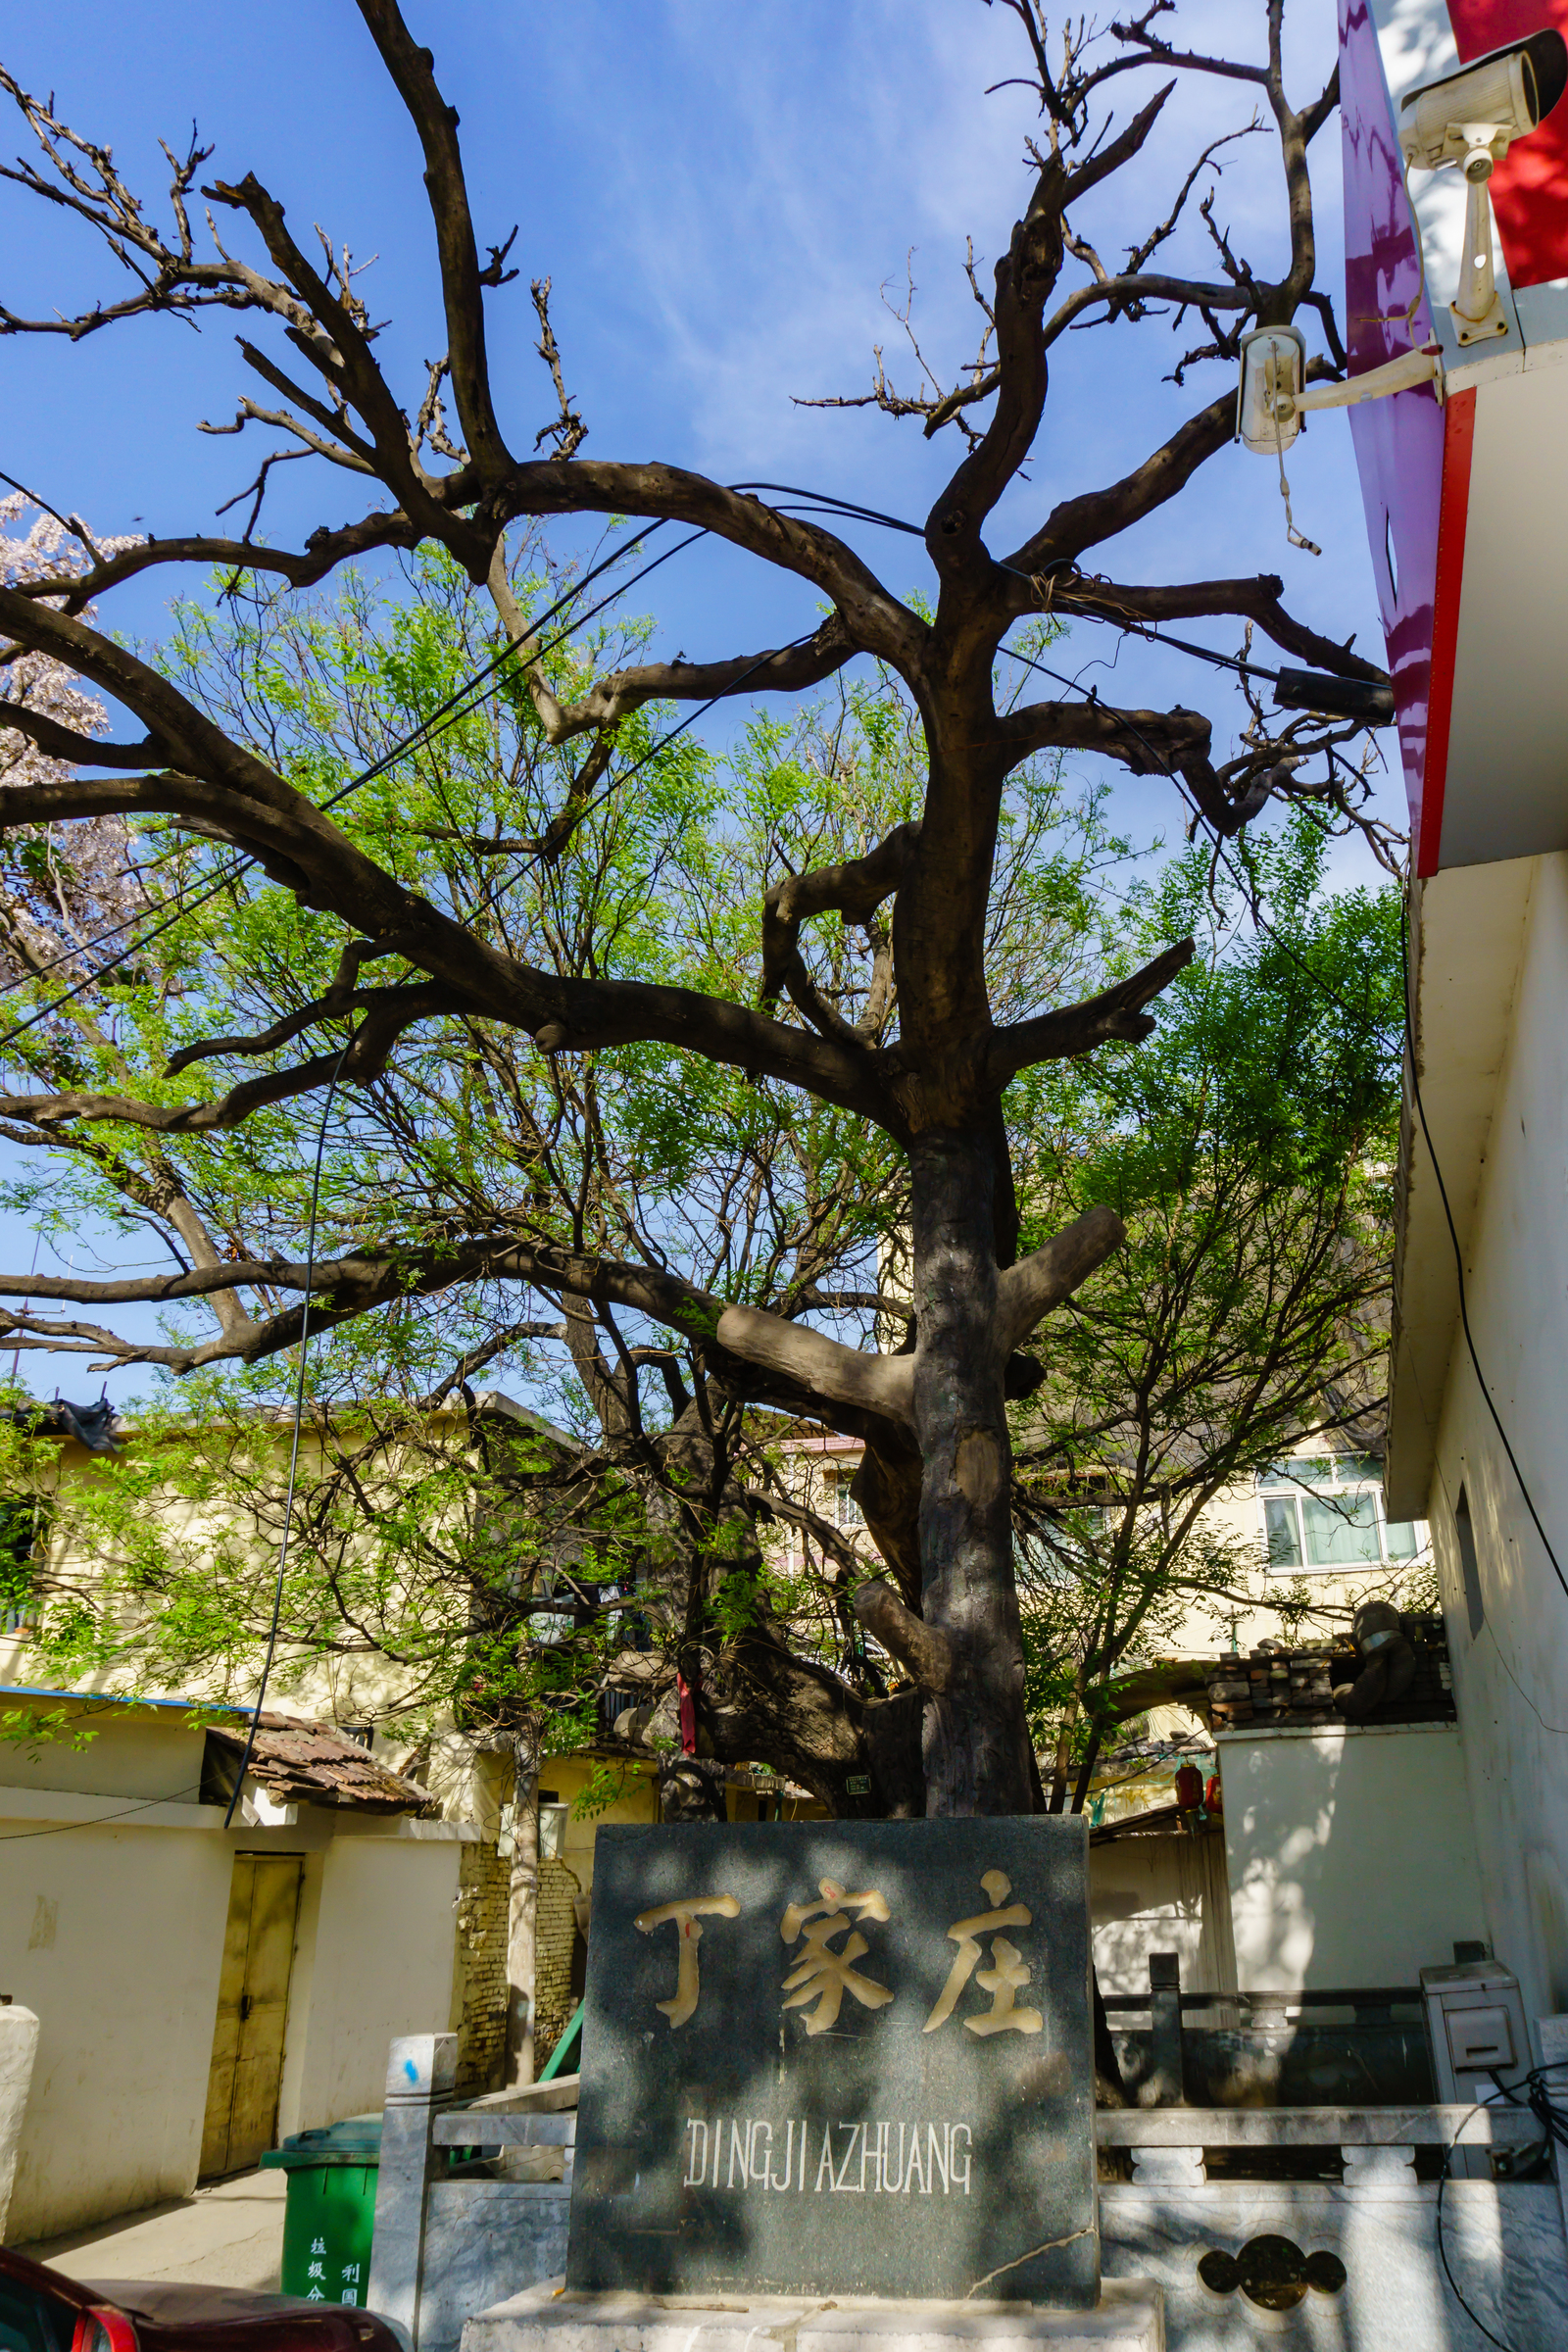
\includegraphics[keepaspectratio, height = 0.6\textheight]{dingjia/cunbei.jpg}
  \caption{丁家庄村碑}
  \label{fig:cunbei}
  % \raggedright
  \raggedright \small 拍摄于2017年4月20日,丁家庄村口的村碑和百年老槐树。
\end{figure}
\clearpage


\dingphotoh{sanbadaji}{熙熙攘攘的三八大集}{拍摄于2017年5月8日,丁家庄每逢农历三、
  八为大集。}{zuwu1}{北侧一处供出租的楼房外景}{拍摄于2017年4月7日。}

\dingphotov{guodao1}{一条街道}{拍摄于2017年4月7日。}

\dingphotoh{guzhai}{城中村最为破败的一间自搭棚户}{拍摄于2017年5月6日,很难想象这
  屋子究竟是属于丁家庄村民还是外来人口。因感无助于对当事人或类似人群的状况改善,
  只能给其带来窘迫,笔者未进行询问。}{bizhezuwu}{笔者田野调查中租住的单间}{拍摄
  于2017年4月25日,这个单价一个月租金240元,网络费30元,居住条件在城中村属于中等
  偏上。}

\dingphotov{chucangshi}{夫妻二人和他们一岁孩子所租住的储藏室}{拍摄于2017年4月15日。}

\dingphotov{cesuo1}{城中村中等水平的简易卫生间}{拍摄于2017年3月31日,这类卫生间多
  为房东所建,常加锁只供其名下租客使用。}

\dingphotoh{yangguang}{阳光}{拍摄于2017年4月26日,木板房为挂锁卫生间。}{lou1}{某
  住房的二三层外墙}{拍摄于2016年11月20日。}

\dingphotov{shaoshui}{丁家庄村民常用的木柴铁皮桶炉}{拍摄于2017年5月8日,丁家庄一
  些村民为节俭持家常用这种简易炉烧开水,火力弱,耗时长、烟雾较大。}

\dingphotoh{youeryuan}{幼儿园外墙与线缆}{拍摄于2017年3月31日。}{wanshua}{玩耍的孩子们}{拍摄于2017年5月7日。}

\dingphotov{jiagai}{改造楼梯、层层加盖的一座楼房}{拍摄于2017年5月11日}

\dingphotoh{jiejing2}{街景}{拍摄于2017年3月26日。}{caishichang}{丁家庄综合市场中
  的一个菜摊位}{拍摄于2017年4月26日,据摊主说,这一个摊位一年租金近9万,塑料袋花
  费近1万。虽然是大棚内的开放式摊位,租金比综合市场中的活动板房小吃店还要高不少。}

\dingphotoh{caitandajie1}{城中村内一处简易搭建的菜摊}{拍摄于2016年12月14日,城中
  村内一个菜摊。区别于综合市场的高租金,这里并无租金。内有被褥,卖菜大姐应当也睡
  在这里。} {caitandajie2}{简易菜摊消失了}{拍摄于2017年3月8日,许是抵不住严寒和收
  入微薄,再看这里时已经不见了卖菜大姐和她的摊位,只有床垫。}

\dingphotoh{zhian}{墙上张贴的治安告示}{拍摄于2017年3月31日,丁家庄外墙上的治安告
  示。这里盗窃案件可能稍高于济南市其他小区,但远未达到恶劣的程度。笔者数十次进进
  出出未曾见过街头吵架、打架。}{diushi}{一位走丢的小孩暂在三轮车摊主的怀抱中睡
  着}{拍摄于2016年11月09日,小孩从城中村北侧的丁家庄综合市场误入城中村,寻不见家
  长大哭不止,后在三轮车饮食摊主怀中睡着,身上披着他人的大衣。}

\dingphotoh{hua1}{一处住户外侧的绿植与杂物}{拍摄于2017年4月12日。}{yangtai}{一处
  阳台——花与衣}{拍摄于2017年4月12日。}

\dingphotov{cbd}{丁家庄工业南路南区一户未拆住房的外墙}{拍摄于2017年4月20日,丁家
  庄南区是第一批拆除的宅基地住房,当时已达成动迁20余户,只余3户尚未动迁。}

% 